
\textit{Available users} are those for which user profile data was successfully collected.  Unavailable users are those for whom an attempt to acquire user attributes resulted in a \textit{404 Not Found} error.  We assume these user accounts are closed.\\ 
\begin{tabular}[t]{| l | l |}
\hline
Users & 17,688,493  \\ \hline
Available Users & 17,475,570 (98.8\%) \\ \hline
Unavailable Users & 212,923 (1.2\%) \\ \hline
Core Users & 242,275 \\ \hline
Available Core Users & 238,323 (98.8\% of core) \\ \hline
Unavailable Core Users & 3,952 (1.2\% of core) \\ \hline
\end{tabular}

\subsection{Subgraphs}
\textit{Graph edges} refers to the connections between core users and any other user.\\\\
\begin{tabular}{| l | l | }
\hline
Users is Subgraph 1 & 15,548,091 \\ \hline
Available Users is Subgraph 1 & 15,363,277 \\ \hline
Core Users in Subgraph 1  & 194,004 \\ \hline
Remaining Core Users  & 48,267 \\ \hline
Remaining Subgraphs  & 46,403 \\ \hline
Connections to Subgraph 1  & 46,924 \\ \hline
Total Connected Users & 240,932 \\ \hline
\end{tabular}

\subsection{Boolean User Attributes}
Attributes whose values are either \textit{true} or \textit{false}.\\\\
\begin{tabular}{| l | l | l |}
\hline
\textbf{Attribute} & \textbf{\# True (Core)} & \textbf{\% True (Core)} \\ \hline
Protected & 8,517 & 3.575  \\ \hline
Geo-Enabled & 58,432 & 24.518 \\ \hline
Verified & 119 & 0.050 \\ \hline
Contributors Enabled & 7 & 0.003 \\ \hline
Show All Inline Media & 18,870 & 7.918 \\ \hline
URL & 118,364 & 49.665 \\ \hline
Is Translator & 72 & 0.030 \\ \hline
\end{tabular}

\subsection{Enumerated User Attributes}
Attributes for which there are a relatively small number of values, other than boolean values.
\subsubsection{Language}
Percentage of users per language.\\\\
\begin{tabular}{| l | l | l | l | }
\hline
\textbf{Language Code} & \textbf{Language} & \textbf{\# (Core)}  & \textbf{\% (Core)} \\ \hline
en & English & 173,782 & 72.919 \\ \hline
ja & Japanese & 44,499 & 18.672 \\ \hline
es & Spanish & 16,210 & 6.802 \\ \hline
de & German & 1,560 & 0.655 \\ \hline
fr & French & 1,222 & 0.513 \\ \hline
it & Italian & 713 & 0.299 \\ \hline
ko & Korean & 337 & 0.141 \\ \hline
\end{tabular}

\subsubsection{UTC Offset}
\begin{tabular}{| l | l | l |}
\hline
\textbf{UTC Offset} & \textbf{\# (Core)} & \textbf{\% (Core)} \\ \hline
(none)	&	38287	&	16.065	\\ \hline
32400	&	36551	&	15.337	\\ \hline
-18000	&	26196	&	10.992	\\ \hline
-10800	&	25001	&	10.490	\\ \hline
-28800	&	23344	&	9.795	\\ \hline
-21600	&	17830	&	7.481	\\ \hline
-14400	&	12698	&	5.328	\\ \hline
25200	&	10425	&	4.374	\\ \hline
-36000	&	10162	&	4.264	\\ \hline
3600	&	9607	&	4.031	\\ \hline
0	&	7067	&	2.965	\\ \hline
-25200	&	4360	&	1.829	\\ \hline
28800	&	4065	&	1.706	\\ \hline
-32400	&	3573	&	1.499	\\ \hline
-16200	&	2685	&	1.127	\\ \hline
7200	&	1908	&	0.801	\\ \hline
36000	&	1286	&	0.540	\\ \hline
10800	&	1054	&	0.442	\\ \hline
19800	&	717	&	0.301	\\ \hline
43200	&	322	&	0.135	\\ \hline
-39600	&	236	&	0.099	\\ \hline
14400	&	213	&	0.089	\\ \hline
18000	&	163	&	0.068	\\ \hline
12600	&	138	&	0.058	\\ \hline
34200	&	103	&	0.043	\\ \hline
-7200	&	100	&	0.042	\\ \hline
21600	&	91	&	0.038	\\ \hline
-12600	&	57	&	0.024	\\ \hline
46800	&	24	&	0.010	\\ \hline
-3600	&	20	&	0.008	\\ \hline
39600	&	19	&	0.008	\\ \hline
16200	&	9	&	0.004	\\ \hline
23400	&	7	&	0.003	\\ \hline
20700	&	5	&	0.002	\\ \hline
\end{tabular}
\vspace{2.5in}

\subsubsection{Time Zone}
Only the top 100 time zones are shown here.\\
\begin{tabular}{| l | l | l | l | l | l |}
\hline
\textbf{Time Zone} & \textbf{\# (Core)} & \textbf{\% (Core)} & \textbf{Time Zone} & \textbf{\# (Core)} & \textbf{\% (Core)} \\ \hline
(none)	&	38287	&	16.065	&	Kyiv	&	215	&	0.090	\\ \hline
Tokyo	&	30332	&	12.727	&	Brussels	&	214	&	0.090	\\ \hline
Pacific Time (US \& Canada)	&	23280	&	9.768	&	Monterrey	&	214	&	0.090	\\ \hline
Brasilia	&	15997	&	6.712	&	Lima	&	194	&	0.081	\\ \hline
Central Time (US \& Canada)	&	15327	&	6.431	&	Copenhagen	&	183	&	0.077	\\ \hline
Eastern Time (US \& Canada)	&	15066	&	6.322	&	Riyadh	&	178	&	0.075	\\ \hline
Santiago	&	12131	&	5.090	&	Abu Dhabi	&	173	&	0.073	\\ \hline
Hawaii	&	10162	&	4.264	&	Athens	&	164	&	0.069	\\ \hline
Quito	&	10152	&	4.260	&	Bucharest	&	151	&	0.063	\\ \hline
Jakarta	&	9334	&	3.917	&	West Central Africa	&	151	&	0.063	\\ \hline
Greenland	&	7968	&	3.343	&	Warsaw	&	148	&	0.062	\\ \hline
London	&	5968	&	2.504	&	Perth	&	145	&	0.061	\\ \hline
Mountain Time (US \& Canada)	&	3826	&	1.605	&	Chennai	&	144	&	0.060	\\ \hline
Amsterdam	&	3600	&	1.511	&	Auckland	&	139	&	0.058	\\ \hline
Alaska	&	3573	&	1.499	&	Tehran	&	138	&	0.058	\\ \hline
Osaka	&	3509	&	1.472	&	Guadalajara	&	133	&	0.056	\\ \hline
Caracas	&	2685	&	1.127	&	Cairo	&	130	&	0.055	\\ \hline
Seoul	&	1912	&	0.802	&	Vienna	&	126	&	0.053	\\ \hline
Mexico City	&	1829	&	0.767	&	Wellington	&	124	&	0.052	\\ \hline
Singapore	&	1677	&	0.704	&	Kuwait	&	122	&	0.051	\\ \hline
Berlin	&	1494	&	0.627	&	Jerusalem	&	117	&	0.049	\\ \hline
Madrid	&	1160	&	0.487	&	Budapest	&	115	&	0.048	\\ \hline
Paris	&	1106	&	0.464	&	Bern	&	114	&	0.048	\\ \hline
Buenos Aires	&	1008	&	0.423	&	Mid-Atlantic	&	100	&	0.042	\\ \hline
Bangkok	&	1000	&	0.420	&	Helsinki	&	96	&	0.040	\\ \hline
Kuala Lumpur	&	944	&	0.396	&	Riga	&	93	&	0.039	\\ \hline
Sapporo	&	762	&	0.320	&	Adelaide	&	91	&	0.038	\\ \hline
Hong Kong	&	627	&	0.263	&	Hanoi	&	73	&	0.031	\\ \hline
Moscow	&	595	&	0.250	&	St. Petersburg	&	73	&	0.031	\\ \hline
Rome	&	594	&	0.249	&	Belgrade	&	71	&	0.030	\\ \hline
Sydney	&	562	&	0.236	&	Nairobi	&	66	&	0.028	\\ \hline
Bogota	&	526	&	0.221	&	Tijuana	&	64	&	0.027	\\ \hline
Istanbul	&	474	&	0.199	&	Casablanca	&	63	&	0.026	\\ \hline
Arizona	&	455	&	0.191	&	Ekaterinburg	&	63	&	0.026	\\ \hline
Edinburgh	&	411	&	0.172	&	Prague	&	62	&	0.026	\\ \hline
Beijing	&	399	&	0.167	&	Newfoundland	&	57	&	0.024	\\ \hline
Melbourne	&	396	&	0.166	&	Minsk	&	54	&	0.023	\\ \hline
Dublin	&	362	&	0.152	&	Sofia	&	51	&	0.021	\\ \hline
Stockholm	&	357	&	0.150	&	Islamabad	&	49	&	0.021	\\ \hline
Atlantic Time (Canada)	&	339	&	0.142	&	Kolkata	&	49	&	0.021	\\ \hline
New Delhi	&	304	&	0.128	&	Canberra	&	48	&	0.020	\\ \hline
Central America	&	301	&	0.126	&	Fiji	&	46	&	0.019	\\ \hline
Pretoria	&	275	&	0.115	&	Chihuahua	&	44	&	0.018	\\ \hline
Indiana (East)	&	258	&	0.108	&	Harare	&	44	&	0.018	\\ \hline
Lisbon	&	243	&	0.102	&	Karachi	&	43	&	0.018	\\ \hline
Taipei	&	231	&	0.097	&	Zagreb	&	39	&	0.016	\\ \hline
La Paz	&	228	&	0.096	&	Yakutsk	&	36	&	0.015	\\ \hline
Brisbane	&	225	&	0.094	&	Mazatlan	&	35	&	0.015	\\ \hline
Mumbai	&	220	&	0.092	&	Novosibirsk	&	32	&	0.013	\\ \hline
International Date Line West	&	216	&	0.091	&	Georgetown	&	28	&	0.012	\\ \hline
\end{tabular}

\onecolumn
\subsubsection{Status Source}
Source of the most recent tweet.  Only the top 50 sources are included here.\\\\
 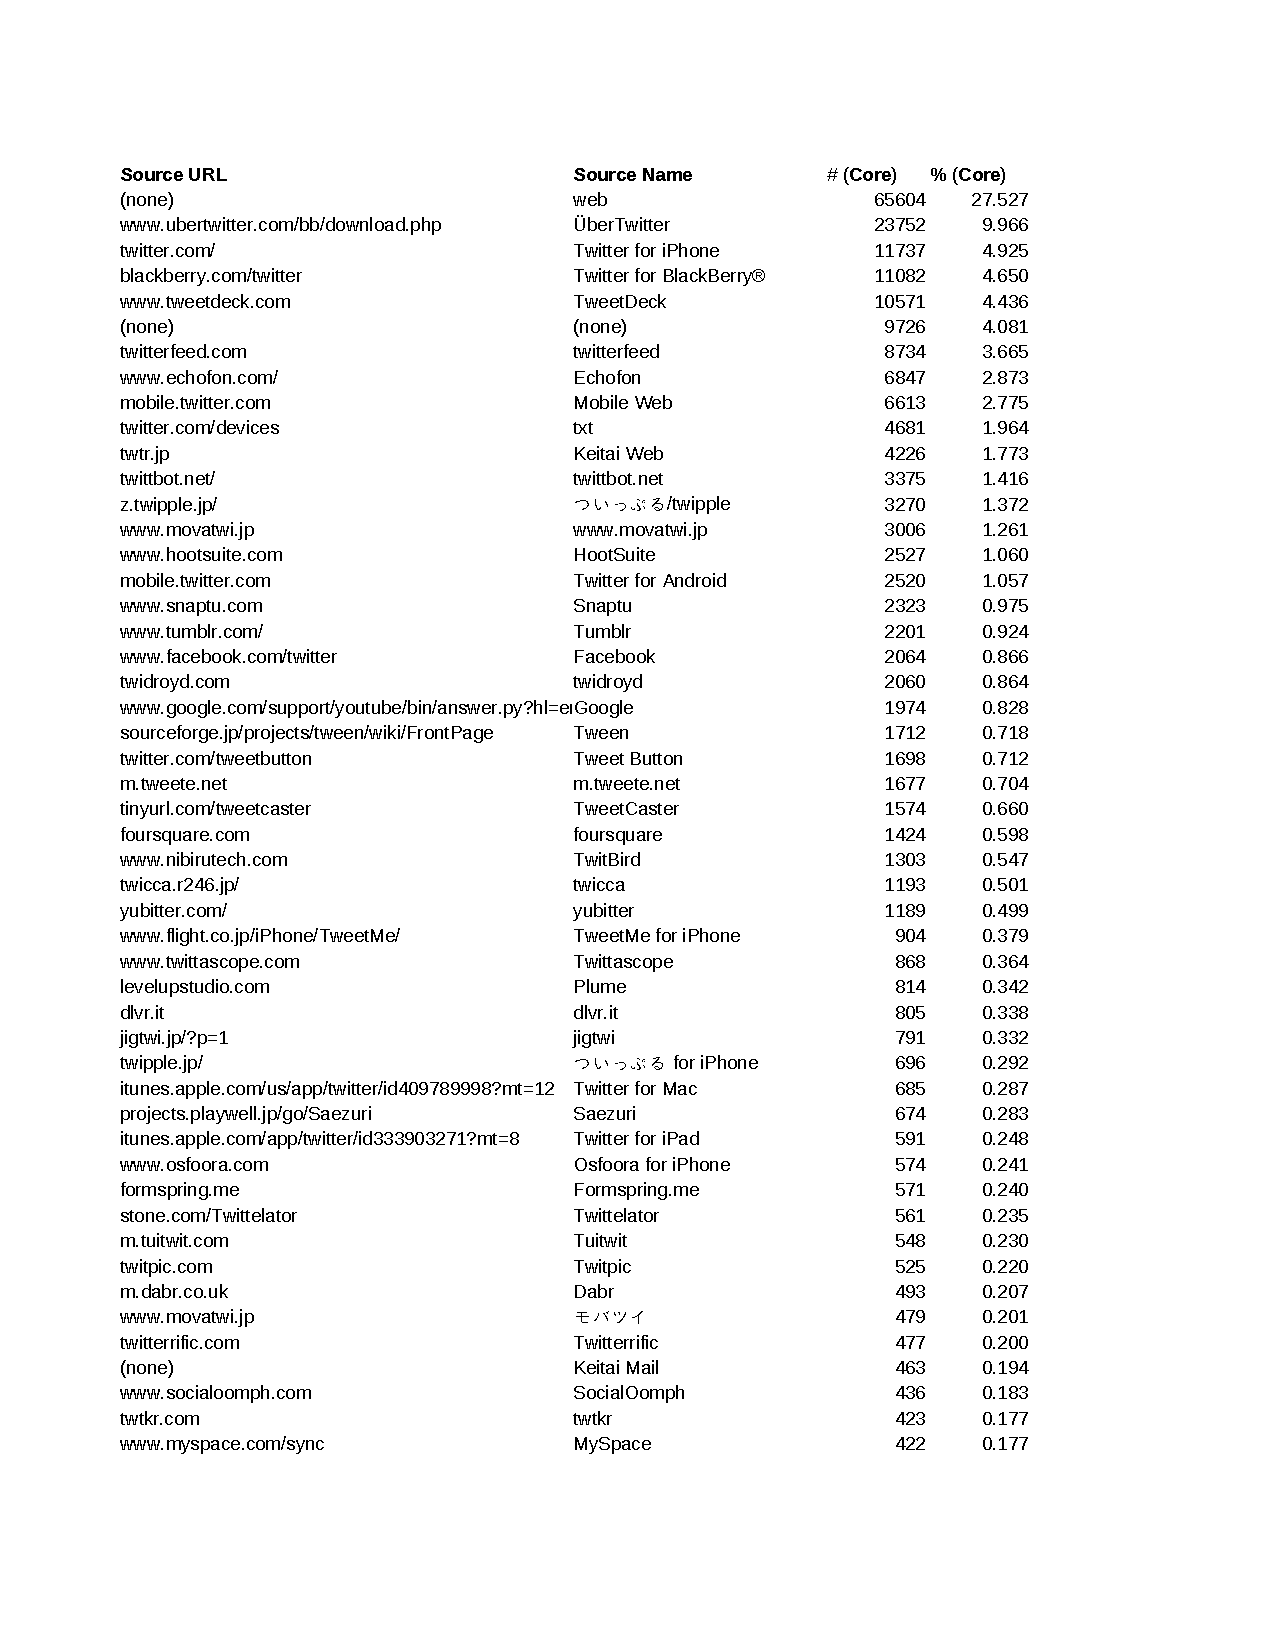
\includegraphics[width=6in]{sources.pdf}

\twocolumn
\subsection{Location}
\noindent Location data is entered free-form.  That is, a user can set their location field to anything they want.  In order to use the location data, we need to figure out which locations are not valid, and we need to transform valid locations into a format that can be processed.  For example, we want all users from San Francisco to have a location attribute of \textit{San Francisco, CA, USA}, so that we can easily determine which users share a location.  We are using the Google Maps Geocoding API to make this conversion.  When the API returns more than one result, we can either remove those location from our analysis, try a different method of processing, or try to determine the commonality between multiple results (if, for example, all results are in France, we can use France in our analysis).  When the API returns zero results, we cannot use the location data.\\\\
The Geocoding API has some amount of error.  The returned results are not always a correct transformation of the original location.  We cannot manually examine each result for error, but we do plan to look at a subset of the results and derive a general error rate from that sample.\\\\
The Geocoding API is rate-limited to 2,500 queries per day per IP address.  Google Maps API Premier members can query up to 100,000 per day, but that service starts at \$10,000, so is probably beyond the budget of this project. Yahoo also has a Geocoding API, to which we can make 5,000 calls per day.  However, we would prefer not to complicate the data collection by using both Google and Yahoo services.\\\\
Rate-limiting of Geocoding queries is an issue we need to address urgently.  We either need to find a way to make more requests to the API without breaking the terms of service, or we need to get the information from the Google or Yahoo front-end.  Alternatively, we could design our own location-conversion script, but we see this as non-ideal.

